\myheader{Solution}{Assignment 7}{Internet Architecture}
\myquestion{Autonomous System (AS)}

Please answer the following questions about \textit{dynamic routing} based 
on the following topology:

\begin{figure}[H]
    \begin{center}
        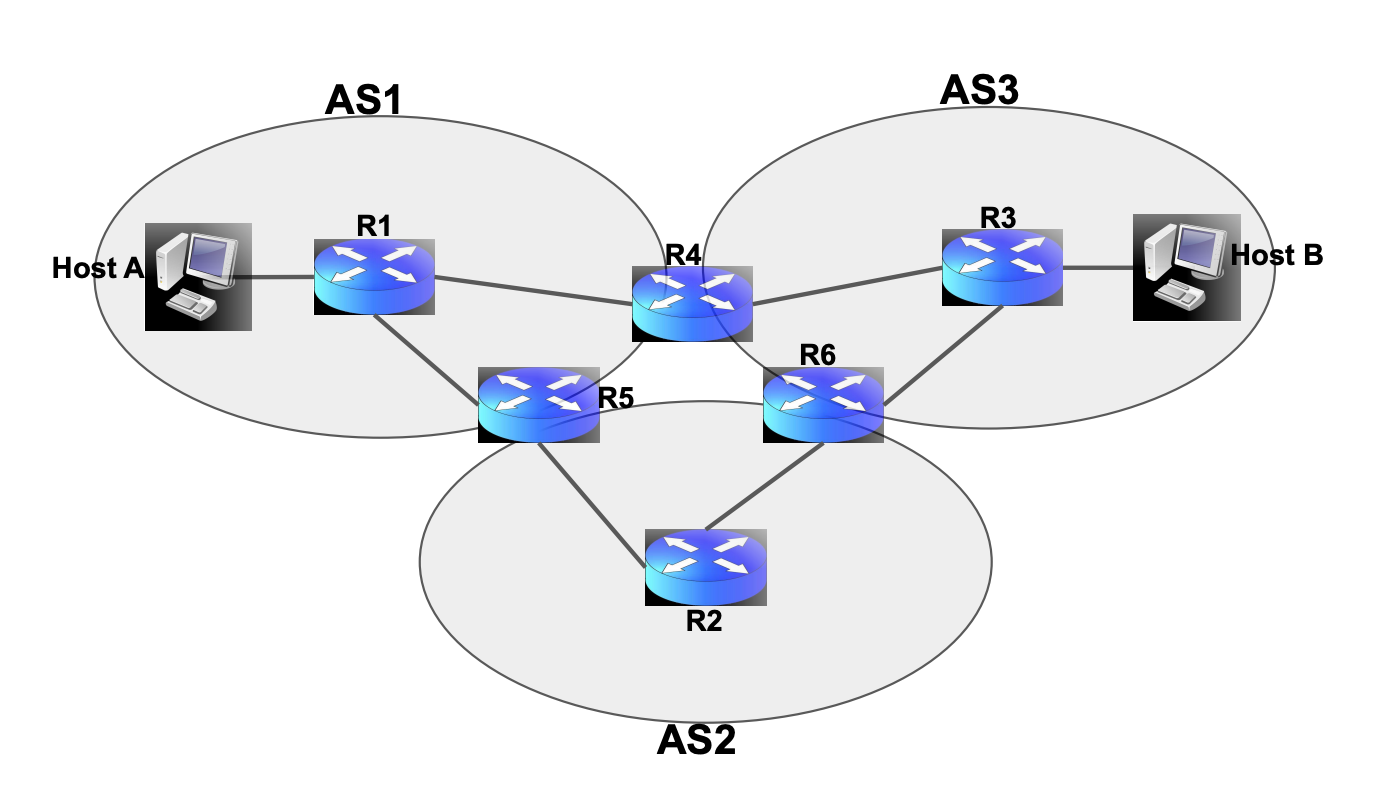
\includegraphics[scale=0.25]{q2.png}
        \caption{Sample topology.}
        \label{fig:q2.png}
    \end{center}
\end{figure}

%----------------------------------------------------------------------------------------------
% Q2.a
%----------------------------------------------------------------------------------------------
\begin{enumerate}
    \item
Please provide a list of routing protocols (or protocol families) that are at least required for each
router such that every router can obtain a route to all devices (i.e., hosts or routers). Assume
that there are no static routes. Justify your answer.
\end{enumerate}

\begin{tcolorbox}
    \mysolution{} 
    Here's a list of routing protocols that are required for routers in the network such that 
    every router can obtain a route to all devices. 
    \begin{itemize}
        \item Intra-AS routing protocol for AS1
        \item Intra-AS routing protocol for AS2
        \item Intra-AS routing protocol for AS3
        \item Inter-AS routing protocol
    \end{itemize}
\end{tcolorbox}

%----------------------------------------------------------------------------------------------
% Q2.b
%----------------------------------------------------------------------------------------------
\begin{enumerate}
    \setcounter{enumi}{1}
    \item
    Suppose Host A wants to communicate with Host B. Despite the potentially longer AS Path,
AS1 wants AS3 to route traffic via AS2. List three different ways in which AS1 might achieve
that goal. In addition, provide three different reasons why AS 1 might have chosen this policy.
\end{enumerate}

\begin{tcolorbox}
    \mysolution{} \\
    \begin{itemize}
        \item The capacity of the link that connects AS1 and AS3 directly might be not sufficient
            to handle all packets from AS1 to AS3 and vice versa. 
        \item It might be the case that direct connection between AS1 and AS3 has more number of
            intermediate routers than a path which goes through AS2. 
        \item AS2 might apply some security policies to packets, such that DDoS attacks are 
            prevented. 
    \end{itemize}
\end{tcolorbox}

%----------------------------------------------------------------------------------------------
% Q2.c
%----------------------------------------------------------------------------------------------
\begin{enumerate}
    \setcounter{enumi}{2}
    \item
    Do host A and host B need to speak BGP? Why/Why not?
\end{enumerate}

\begin{tcolorbox}
    \mysolution{} \\
    No, there is no need for host A and host B to speak BGP. In fact these hosts send their 
    packet to the first router they are connected to and these router speak BGP in order
    to be able to steer packets in the right direction. 
\end{tcolorbox}


%----------------------------------------------------------------------------------------------
% Q2.d
%----------------------------------------------------------------------------------------------
\begin{enumerate}
    \setcounter{enumi}{3}
    \item
When running continiously pings for 5 minutes from Host B to Host A, AS3 noticed that RTTs
via the direct link between AS1 and AS3 are higher than RTTs observed when using the route
via AS2. Why may this happen? Provide, and explain, two different reasons. Do you expect
those reasons to have transient or long-lasting effects?
\end{enumerate}

\begin{tcolorbox}
    \mysolution{} \\
    \begin{itemize}
        \item The capacity of the link that connects AS1 and AS3 directly might be lower 
            comparing to the capacity of routers in the path from AS1 to AS2 and AS2 to AS3.
        \item It might be the case that direct connection between AS1 and AS3 has more number of
            intermediate routers than a path which goes through AS2. 
    \end{itemize}
\end{tcolorbox}



